\documentclass{beamer}\usepackage[]{graphicx}\usepackage[]{color}
%% maxwidth is the original width if it is less than linewidth
%% otherwise use linewidth (to make sure the graphics do not exceed the margin)
\makeatletter
\def\maxwidth{ %
  \ifdim\Gin@nat@width>\linewidth
    \linewidth
  \else
    \Gin@nat@width
  \fi
}
\makeatother

\definecolor{fgcolor}{rgb}{1, 0.894, 0.769}
\newcommand{\hlnum}[1]{\textcolor[rgb]{0.824,0.412,0.118}{#1}}%
\newcommand{\hlstr}[1]{\textcolor[rgb]{1,0.894,0.71}{#1}}%
\newcommand{\hlcom}[1]{\textcolor[rgb]{0.824,0.706,0.549}{#1}}%
\newcommand{\hlopt}[1]{\textcolor[rgb]{1,0.894,0.769}{#1}}%
\newcommand{\hlstd}[1]{\textcolor[rgb]{1,0.894,0.769}{#1}}%
\newcommand{\hlkwa}[1]{\textcolor[rgb]{0.941,0.902,0.549}{#1}}%
\newcommand{\hlkwb}[1]{\textcolor[rgb]{0.804,0.776,0.451}{#1}}%
\newcommand{\hlkwc}[1]{\textcolor[rgb]{0.78,0.941,0.545}{#1}}%
\newcommand{\hlkwd}[1]{\textcolor[rgb]{1,0.78,0.769}{#1}}%
\let\hlipl\hlkwb

\usepackage{framed}
\makeatletter
\newenvironment{kframe}{%
 \def\at@end@of@kframe{}%
 \ifinner\ifhmode%
  \def\at@end@of@kframe{\end{minipage}}%
  \begin{minipage}{\columnwidth}%
 \fi\fi%
 \def\FrameCommand##1{\hskip\@totalleftmargin \hskip-\fboxsep
 \colorbox{shadecolor}{##1}\hskip-\fboxsep
     % There is no \\@totalrightmargin, so:
     \hskip-\linewidth \hskip-\@totalleftmargin \hskip\columnwidth}%
 \MakeFramed {\advance\hsize-\width
   \@totalleftmargin\z@ \linewidth\hsize
   \@setminipage}}%
 {\par\unskip\endMakeFramed%
 \at@end@of@kframe}
\makeatother

\definecolor{shadecolor}{rgb}{.97, .97, .97}
\definecolor{messagecolor}{rgb}{0, 0, 0}
\definecolor{warningcolor}{rgb}{1, 0, 1}
\definecolor{errorcolor}{rgb}{1, 0, 0}
\newenvironment{knitrout}{}{} % an empty environment to be redefined in TeX

\usepackage{alltt}
\usepackage{../371g-slides}
% Uncomment these lines to print notes pages
% \pgfpagesuselayout{4 on 1}[letterpaper,border shrink=5mm,landscape]
% \setbeameroption{show only notes}
\title{Introduction to R}
\subtitle{Lecture 2}
\author{STA 371G}
\IfFileExists{upquote.sty}{\usepackage{upquote}}{}
\begin{document}



  \frame{\maketitle}

  % Show outline at beginning of each section
  \AtBeginSection[]{
    \begin{frame}<beamer>
      \tableofcontents[currentsection]
    \end{frame}
  }

  %%%%%%% Slides start here %%%%%%%

  \begin{darkframes}
  
  
  
    \begin{frame}{Again, what is R? What is RStudio?}
    \fontsize{10}{10}\selectfont
     R is the language, which we access through RStudio (interface).\pause   
     
     \bigskip
     Here is what it looks like... 

      \begin{center}
        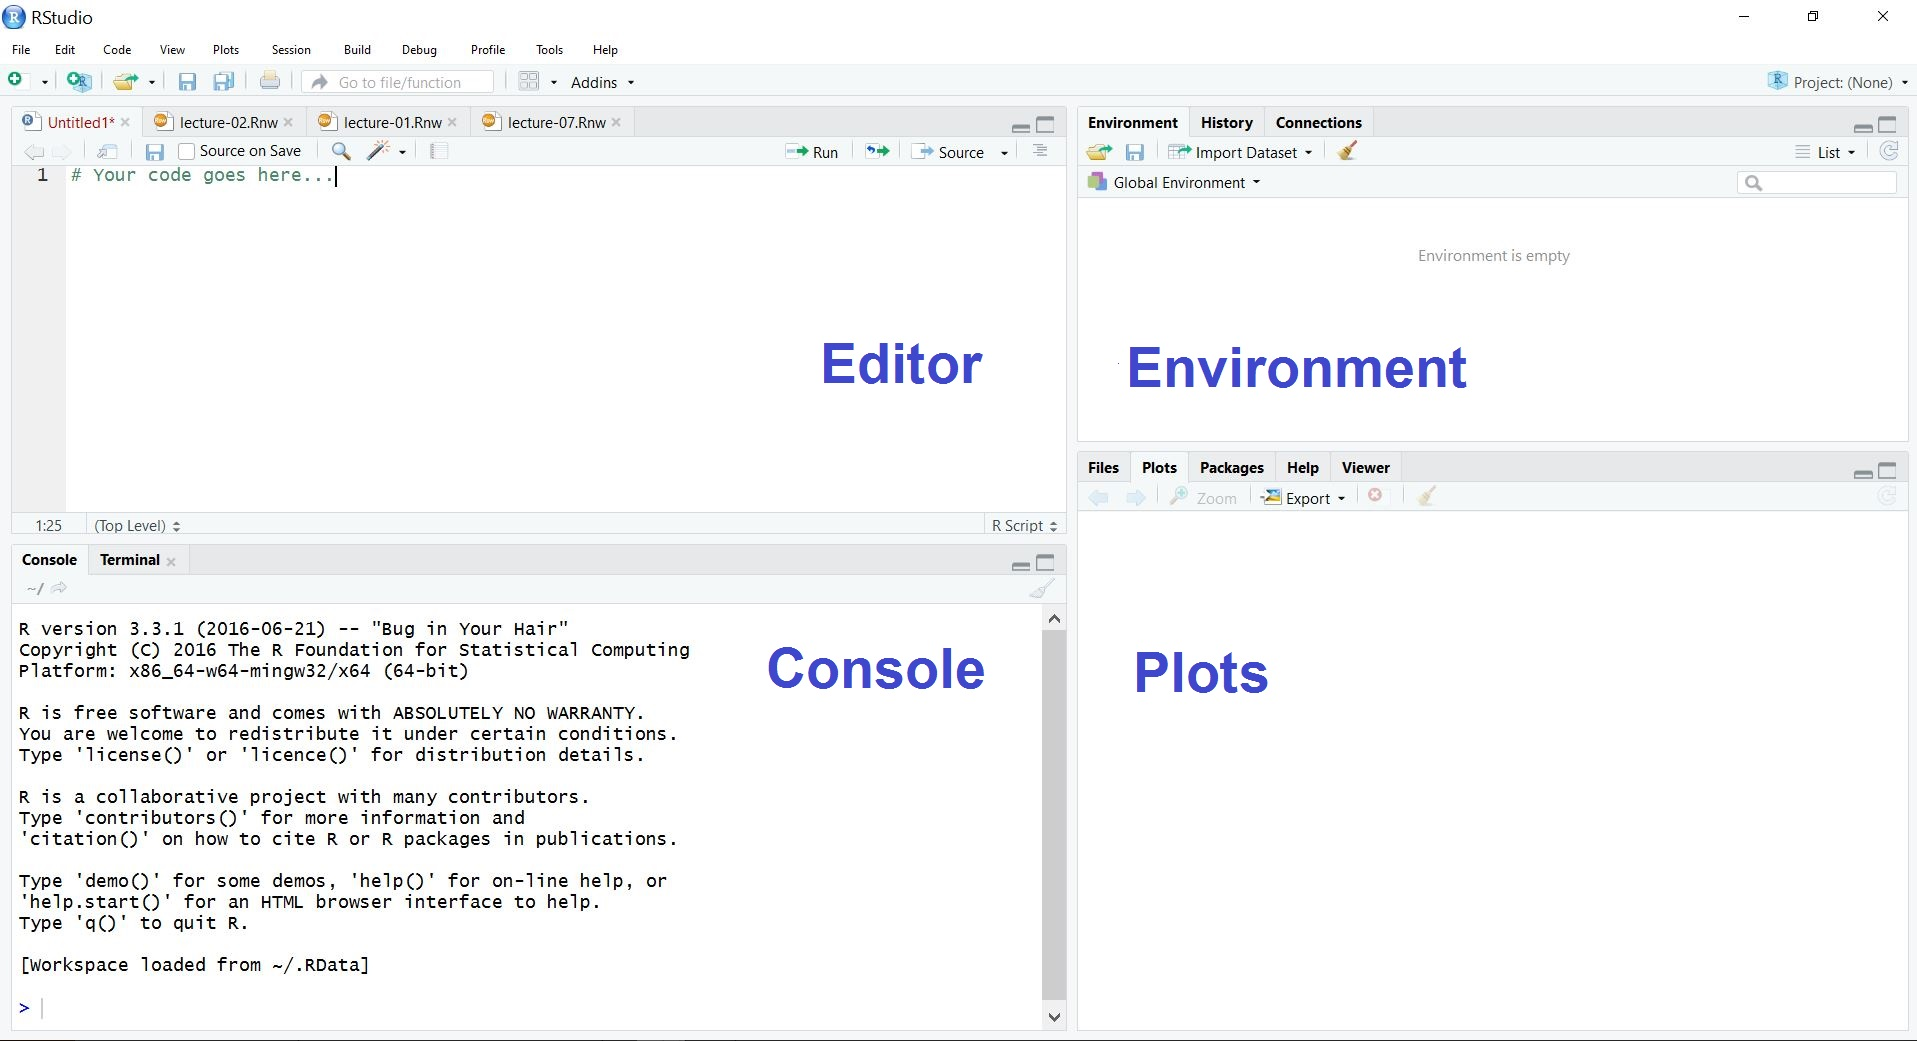
\includegraphics[width=4in]{RStudio}
      \end{center} \pause
    \end{frame}

    
    
    \begin{frame}{RStudio Layout}
    \fontsize{10}{10}\selectfont
      \begin{itemize}
        \item \alert{Console:} This is where calculations/code are passed to R and results are observed. \pause
        \item \alert{Editor:} It is not practical to write long calculations/code in console. We write them in the editor, and "Run" to pass to the console. \pause
        \item \alert{Environment:} All data sets/variables we define can be found here. \pause
        \item \alert{Plots:} When we plot things, they will first appear here.
      \end{itemize} 
    \end{frame}
    
    
    
    
    \begin{frame}{Let's get started...}
    \fontsize{10}{10}\selectfont
    Assume you want to calculate your course grade.
    
      \begin{table}[!b]
        {\carlitoTLF % Use monospaced lining figures
        \begin{tabularx}{\textwidth}{ccc}
           
           Assignment & Weight  & Grade \\ 
          \toprule
            Class participation & 5\%	&	91  \\
            Reading assignments & 5\%	&	95  \\
            Homework    & 15\%	&	 86 \\
            Project     & 15\%	&	 83 \\
            Midterm 1   & 20\%	&	 88 \\
            Midterm 2   & 20\%	&	 76 \\
            Final exam  & 20\%	&	 84 \\
        \end{tabularx}}
        
      \end{table} 
    \end{frame}


    \begin{frame}[fragile]{Using the console}
      First try this in console.
\begin{knitrout}
\definecolor{shadecolor}{rgb}{0.137, 0.137, 0.137}\begin{kframe}
\begin{alltt}
\hlnum{0.05} \hlopt{*} \hlnum{91} \hlopt{+} \hlnum{0.05} \hlopt{*} \hlnum{95} \hlopt{+} \hlnum{0.15} \hlopt{*} \hlnum{86} \hlopt{+} \hlnum{0.15} \hlopt{*} \hlnum{83} \hlopt{+} \hlnum{0.2} \hlopt{*}
    \hlnum{88} \hlopt{+} \hlnum{0.2} \hlopt{*} \hlnum{76} \hlopt{+} \hlnum{0.2} \hlopt{*} \hlnum{84}
\end{alltt}
\begin{verbatim}
[1] 84.25
\end{verbatim}
\end{kframe}
\end{knitrout}
      \pause
      It makes sense to save the result to a variable to be able to use later.
\begin{knitrout}
\definecolor{shadecolor}{rgb}{0.137, 0.137, 0.137}\begin{kframe}
\begin{alltt}
\hlstd{my371} \hlkwb{<-} \hlnum{0.05} \hlopt{*} \hlnum{91} \hlopt{+} \hlnum{0.05} \hlopt{*} \hlnum{95} \hlopt{+} \hlnum{0.15} \hlopt{*} \hlnum{86} \hlopt{+} \hlnum{0.15} \hlopt{*}
    \hlnum{83} \hlopt{+} \hlnum{0.2} \hlopt{*} \hlnum{88} \hlopt{+} \hlnum{0.2} \hlopt{*} \hlnum{76} \hlopt{+} \hlnum{0.2} \hlopt{*} \hlnum{84}
\end{alltt}
\end{kframe}
\end{knitrout}
    \end{frame}



    \begin{frame}[fragile]{Using the editor}
      \fontsize{10}{10}\selectfont
      It much convenient to do the calculations/coding in the editor and then "run" them. \pause
      
      Working with vectors is also common, which are simply data containers.

\begin{knitrout}
\definecolor{shadecolor}{rgb}{0.137, 0.137, 0.137}\begin{kframe}
\begin{alltt}
\hlcom{# This is the same calculation, using vectors.}
\hlstd{weights} \hlkwb{<-} \hlkwd{c}\hlstd{(}\hlnum{0.05}\hlstd{,} \hlnum{0.05}\hlstd{,} \hlnum{0.15}\hlstd{,} \hlnum{0.15}\hlstd{,} \hlnum{0.2}\hlstd{,} \hlnum{0.2}\hlstd{,} \hlnum{0.2}\hlstd{)}
\hlstd{grades} \hlkwb{<-} \hlkwd{c}\hlstd{(}\hlnum{91}\hlstd{,} \hlnum{95}\hlstd{,} \hlnum{86}\hlstd{,} \hlnum{83}\hlstd{,} \hlnum{88}\hlstd{,} \hlnum{76}\hlstd{,} \hlnum{84}\hlstd{)}
\hlstd{weighted_grades} \hlkwb{<-} \hlstd{weights} \hlopt{*} \hlstd{grades}
\hlstd{my371} \hlkwb{<-} \hlkwd{sum}\hlstd{(weighted_grades)}
\end{alltt}
\end{kframe}
\end{knitrout}
      The multiplication is element-wise. \pause
      
      ``sum'' is a predefined function in R, which sums all the elements in a vector.
  
      \note{Discuss why it makes sense to vectorize and save in variables. We can, for example, use weights in multiple places.}

    \end{frame}
    
    
    
    \begin{frame}[fragile]{Getting help}
      \fontsize{10}{10}\selectfont
      So we used sum function. How can we learn more about its usage and options? \pause
      \bigskip
      
      R has a help command that gives all the details about R functions & packages. \pause
      
      \bigskip
      Simply type "help(sum)" in the console...
    
    
    \end{frame}
    
    
    

  \end{darkframes}

\end{document}
